\chapter{Data Transformations}\label{chap:FormatDecisions}

On today's high performance architectures, using the memory hierarchy effectively is a great challeng with a great reward.
When performance considerations --- architecture, memory hierarchy configuration, even input data characteristics --- are hard-coded into the application, improved memory performance comes at the cost of maintainability and portability.
This is especially relevant for schedule and data optimizations that are applied across loops, where the optimization obscures the underlying operation of the code.
To address this problem, performance portability libraries like RAJA, Kokkos, and YAKL provide abstractions for controlling how loops are scheduled/parallelized and how data is laid out initially. 
However, they do not support changing data layouts between loops without significant manual intervention.
This chapter's focus is on data layout transformations among canonical data layouts and the challenges inherent in enabling their high-level control within performance portability libraries, using RAJA as an example.
First, I introduce programming abstractions into the RAJA library to collect and apply data format transformations between kernels.
Then, I incorporate a built-in performance model for as-automated-as-desired transformation selection. 
Finally, to support key computations that benefit from these layout transformations, I extend RAJA's iteration space description to support loops with non-rectangular iteration spaces.
I also describe how the system could be used in a production code base to amortize modeling costs over multiple executions of the same program.
For computations with sufficiently large data sizes, this approach achieves similar performance to hand-implemented data layout optimizations with significantly fewer code changes across six key benchmark kernels.

\section{Introduction}

The gap between CPU speeds and memory latency recurs throughout computing history, prompting ever-more complex architectural solutions.
From the 384 byte ``B-store'' of the 1960 Ferranti Atlas~\cite{ferranti1960features} to the multi-level cache systems of today, memory hierarchy has endured as the solution.
The challenge is handed from the architect to the programmer, who must write programs that make use of this hierarchy efficiently.
There are two ways of doing this: changing the order in which data is accessed (loop schedules) and changing the order in which data is stored (data layouts).
The previous chapter focused on schedule transformations across multiple loops. 
This chapter focuses on runtime data layout transformations among canonical data layouts.

%Motivate the incorporation of data layout optimizations into PPLs
When optimizing code by hand, these transformations are onerous to implement.
The original, modularized implementation of a computation is obscured by the changes of implementing the transformation. 
When a code is meant to run on multiple systems or evolve to support new features, these optimizations can end up being more trouble than they are worth, the performance improvement offset by the increased maintenance and porting costs.

Performance portability libraries (PPLs) --- like RAJA~\cite{hornung2014RAJA}, Kokkos~\cite{edwards2014kokkos}, and YAKL~\cite{norman2022portable} --- partially address this problem.
By breaking the description of a computation into separable components, programmers can experiment with different schedules and layouts without obscuring the code's underlying operation.
However, control of the layout of data is limited to a global scope; data cannot be reorganized with different layouts throughout a computation.
Should they wish to change the data layout mid-program, they would have to use multiple arrays for the same data, ensuring that each maintain the correct contents.
The brave soul who chooses this option must still overcome yet another obstacle: selecting the right combination of formats.
Even a modest computation of two loops that use four 2D arrays has more than 200 combinations from which to choose, so trying all possible options quickly becomes infeasible. 

%Motivate the problems that arise from incorporation into PPLs
The transformations under consideration here, for example switching a 2D matrix from column- to row-major storage, are well known.
They have been incorporated as automatic transformations within distributed computing contexts as source-to-source research compilers for High Performance Fortran and Fortran D~\cite{bixby1994automatic,kennedy1995automatic,kennedy1998automatic}.
More recently, others have made efforts to incorporate user control of these transformations in domain-specific languages, such as DL~\cite{sung2012dl}, ExaSlang~\cite{kronawitter2018automatic} and Tiramisu~\cite{baghdadi2019tiramisu}.
These DSLs recognize the importance of giving the programmer control over how the program is optimized. %Significance of user indicating layout
However, both the automated and user-controlled approaches use compilers that are specialized, unstandardized, and in the case of HPF no longer existent.
For codes already written using PPLs, where using a standardized language and production-grade compiler is important, these approaches are not feasible.

%Focus on the challenges
Fortunately, performance portability libraries already contain data abstractions that can form the basis for supporting these transformations.
Still, there remain challenges.
First is enabling programmer control of per-loop data layout without requiring it.
Because necessary program analysis and modeling cannot be done at compile-time without modifying the compiler, it must be done at runtime and amortized or stored for use in subsequent executions.
This leads to the next challenge: the overhead of the analysis and performance modeling must be smaller than the improvements provided by the transformations.
Finally, important computations that benefit from layout changes, like correlation and covariance calculations, have iteration spaces where inner loop bounds depend on outer loop iterators, which is not supported by any of the three PPLs.  %Specific motivation of triangular iteration spaces

%Clear contributions
In this chapter, I present an approach that resolves these problems while balancing user control with automation, inspired by inspector-executor patterns often used in the realm of sparse computations~\cite{saltz1990run,saltz1991multiprocessors,Strout14IPDPS,strout2018sparse}.
I also present an implementation of this approach in the RAJA library.
To provide optional automated layout selection, a runtime performance model uses data access information gathered from symbolic evaluation (see Section~\ref{subsec:accesses}) and microbenchmarking results to solve an optimization problem based on previous approaches~\cite{bixby1994automatic}.
Rather than using an integer linear programming (ILP) formulation, I reduce runtime modeling time by using a nonlinear programming problem instead. 
This chapter makes the following contributions:
\begin{itemize}
\item An interface for combining user-specified layout choices with additional choices based on runtime modeling;
\item An optimization to the runtime benchmarking to increase the reuse of results;
\item An optimization to the model's optimization problem to reduce the number of variables by using a nonlinear formulation instead of a linear one; and 
\item Support for iteration spaces with parametric bounds, which includes triangular iteration spaces and are expanded in Chapter~\ref{chap:SparseRAJA} to support sparse iteration spaces. %connection of symbolic segments to sparse contribution
\end{itemize}

I begin with an overview of performance portability libraries, and RAJA in particular (Section 2).
Then, I expand the iteration space abstractions to support computations with relations between loop dimensions (Section 3).
Next, I introduce an interface for user-specified layout transformations between computations (Section 4).
This interface incorporates optional runtime modeling based on microbenchmarking to augment user choices without overriding them.
I build on existing automated approaches and make two key optimizations: one to reduce the number of model coefficients and one to reduce the number of model variables (Section 5).
Then, I sketch how the \FormatDecisions{} system might be used in a production code base (Scetion 6).
Finally, I evaluate the model's accuracy and performance, as well as the entire system's performance and productivity for six benchmark kernels and one application case study (Section 7).
I then review related work (Section 8), and conclude (Section 9).


\section{Background and Assumptions}

Each of the three PPLs has its own programming model and interface, yet the abstractions present in each have similarities.
Most relevant in this chapter are their respective multi-dimensional data abstractions.
This section reviews those abstractions and the assumptions made about codes that use \FormatDecisions{}.

\subsection{PPL Data Abstractions}

All three PPLs have a core multi-dimensional data abstraction around which the rest of the libraries are developed.
In Kokkos and RAJA, the abstraction is the \verb.View..
In YAKL, the abstraction is the \verb.Array..
The key feature shared by these types is that they decouple how the data is referenced from how it is stored.

How exactly the libraries achieve this decoupling differs in both name and method.
In YAKL, \verb.Array. objects have a ``style'' template parameter that indicate if the object should be C style (row-major) or Fortran style (column-major). 
The \verb.View. object in Kokkos also uses a template parameter to specify the mapping of indices to memory.
Kokkos has \verb.LayoutRight. for row-major storage, \verb.LayoutLeft. for column-major, and \verb.LayoutStride. for layouts with arbitrary dimensional strides.
In RAJA, the \verb.View. object is templated by a layout type as well, but the layout type itself does not specify the ordering of the dimensions. 
Instead, layout objects are instantiated at runtime with dimensional orderings and associated with the View when it is initialized.
This chapter is implemented in RAJA, which, combined with limitations of the symoblic evaluation capabilities presented in Chapter 2, lead to some assumptions about codes that use \FormatDecisions{}.

\subsection{Assumptions}
The \FormatDecisions{} system makes the following assumptions/requirements about the user program:
\begin{itemize}
\item Each array in the program can be modeled independently. \FormatDecisions{} sets up and solves one optimization problem per array and does not model interactions between arrays. For example, using two View objects sharing the same underlying sections of memory are prohibited.
\item Every data access is reachable and exercised by symbolic evaluation. All accesses must be incorporated into the performance model to produce accurate results, and these are identified using symbolic evaluation.
\item Modeled loops bodies do not use use iterators or data accesses as arguments to functions. This is to ensure compatibility with symbolic evaluation.
\item All arrays only use dense, hyper-rectangular data layouts, as \FormatDecisions{} only supports canonical layouts.
\item Modeled arrays have dimensionality less than or equal to six. This is the upper bound for dimensionality found in codes of interest, with six-dimensional data appearing in QCD codes.
\end{itemize}


\section{Parametric Iteration Spaces}

While PPLs break the description of a computation into clear and separable parts, their approaches for representing iteration spaces are limited in expressivity.
The expressivity varies by PPL\@.
Kokkos is limited to iteration spaces composed of contiguous ranges.
YAKL additionally supports noncontiguous dimensions with constant strides.
RAJA is the most expressive, due to its \verb.ListSegment. abstraction, which supports iteration space dimensions with arbitrary lists of index values.
However, while any individual dimension can contain arbitrary values, they can only be composed into a multidimensional iteration space using the cartesian product (e.g., $[a, b, c] \times [1..3] = [(a,1), (a,2), (a,3), (b,1), \dots (c,3)]$).

Computations with iteration space dimensions that change throughout the computation, such as those with triangular iteration spaces, cannot be represented within this framework, nor can they be represented by previous works examining data layout selection~\cite{kennedy1998automatic}. 
Examples of these computations include LU decomposition, Cholesky factorization, and statistical calculations like covariance and correlation.
These are important computations in scientific computing.

To address this limitation in current PPLs and represent iteration spaces with relations between the dimensions, I introduce the \verb.SymbolicSegment. type to the RAJA library, which also forms the basis of the sparse iteration space description framework in Chapter~\ref{chap:SparseRAJA}. 
Unlike the \verb.RangeSegment., which requires integer values for its start, stop, and stride, the \verb.SymbolicSegment. supports bounds expressions that combine other segments with constant values. 
This process involves two elements.
First, the \verb.SymbolicSegment. objects maintain their current value through the execution of a kernel. 
Second, rather than returning a static value, the \verb.begin(). and \verb.end(). methods calculate the start and stop values dynamically based on the expressions used in their construction. 
When execution reaches the beginning of a loop, the symbolic bound expressions are evaluated and a standard \verb.RangeSegment. is instantiated for use in the loop.

Valid bound expressions in the definition of a \verb.SymbolicSegment. can contain numeric constants and previously defined symbolic segments, combined with the four basic arithmetic operators. 
By overloading the arithmetic operators to construct expression trees, the symbolic segments can delay evaluating the bounds of the dimension until that level of the loop nest is reached.
Further, it can \textit{re}-evaluate inner bounds expressions as the outer iterator values change.

This approach evaluates the bounds expressions only at the start of each nesting level, akin to the init-statement of a standard for-loop.
Once the bounds expressions are evaluated, the dimension is treated as a standard contiguous range, but maintains the iterator value within the \verb.SymbolicSegment. object itself.
This allows the value to be used in the evaluation of bounds expressions for deeper nesting levels.

When bounds expressions, like those in Figure~\ref{goodTriangles} contain division operations, evaluating them as integer expressions may lead to unexpected results. 
For example, as a lower bound, the expression \verb_1.5 - iSeg / 2_ resolves to $1$ when \verb.iSeg. has the value $0$. 
This is problematic, as $1$ is not greater than or equal to $1.5 - 0/2$.
The problem persists when expressions are rearranged to contain only integers; \verb.(3 - iSeg) / 2. suffers the same fate.
To address this issue, bounds are evaluated as floating point expressions then cast to integer values based on the bound type.
Lower bounds are cast to their ceiling, while upper bounds are cast to their floor.

Symbolic segments can readily express the triangular iteration spaces found in the computations mentioned above. 
Listing~\ref{triangularComparison} shows how a triangular iteration space written using a C++ nested for-loop is expressed using symbolic segments.

\todo{this paragraph needs work}
\todo{first sentence is unclear what I mean}
To match the interface of RAJA's \verb.RangeSegment., a user defines iteration space dimensions in terms of their bounds, not as arbitrary linear constraints.
This mode of description trades this familiarity for slight limits to expressivity.
Specifically, creating polyhedra with cyclical dependences among their indices, such as those show in Figure~\ref{badShapes}, is not possible with \verb.SymbolicSegments.. 
Polyhedral code generators can convert constraint descriptions into \verb.for.-loop bounds with polyhedral scanning techniques~\cite{pouchet2007iterative,grosser2011polly, benabderrahmane2010polyhedral}, but these generate complicated and non-intuitive bounds expressions like those in Figure~\ref{farkasResult}. 
Adding a \verb.min. and \verb.max. expression to the \verb.SymbolicSegment. interface would technically enable the description of this class of polyhedra.
However, the user would either have to use an external tool to generate the expressions or calculate them by hand.
Because these polyhedra are rare in practice --- not appearing within the benchmarks evaluated here --- I chose to leave this feature as future work.

\todo{summary paragraph}

\begin{figure}
\begin{lstlisting}[caption={Comparison of C++ for-loop and RAJA \texttt{SymbolicSegment} representations of a loop nest with a triangular iteration space.},label=triangularComparison]
//C++ for-loop
for(int i = 0; i < Ni; i++) {
	for(int j = i; j < Nj; j++) { // j starts at i
		... 
	}
}

//RAJA SymbolicSegments
auto iSeg = make_symbolic_segment(0, Ni);
auto jSeg = make_symbolic_segment(iSeg, Nj);
auto segments = make_tuple(iSeg, jSeg);
\end{lstlisting}
\end{figure}






\begin{figure}
\begin{subfigure}{0.4\columnwidth}
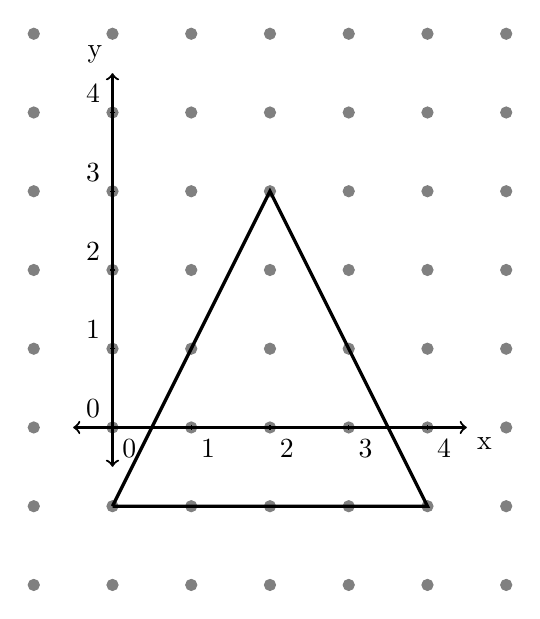
\begin{tikzpicture}
\foreach \x in {-1,0,1,2,3,4,5}
\foreach \i in {-2,-1,0,1,2,3,4,5}
	\filldraw [gray] (\x, \i) circle (2pt);
\draw[thick,<->] (-0.5,0) -- (4.5,0) node[anchor=north west] {x};
\draw[thick,<->] (0,-0.5) -- (0,4.5) node[anchor=south east] {y};
\foreach \x in {0,1,2,3,4}
	\draw (\x cm,1pt) -- (\x cm,-1pt) node[anchor=north west] {$\x$};
\foreach \i in {0,1,2,3,4}
	\draw (1pt,\i cm) -- (-1pt,\i cm) node[anchor=south east] {$\i$};
	
\draw [black, very thick] (0,-1) -- (2,3) -- (4,-1) -- (0,-1);
\end{tikzpicture}
\caption{Graphical depiction of iteration space with dependent $x$ dimension.}\label{triangularIterationSpace1}
\end{subfigure}
\hspace{0.05\columnwidth}
\begin{subfigure}{0.55\columnwidth}
\begin{subfigure}{\columnwidth}
\begin{align}
	-1 \leq &y < 4 \\
	(1 + y) * 0.5 \leq &x \leq (7 - y) * 0.5
\end{align}
\caption{Constraint description of iteration space from~\ref{triangularIterationSpace1}.}\label{constraintDescription1}
\end{subfigure}

\vspace{20pt}

\begin{subfigure}{\columnwidth}
\begin{lstlisting}[]
auto y_seg = make_symbolic_segment(-1,4);
auto x_seg = make_symbolic_segment_inclusive(
							(y_seg + 1) * 0.5, 
							(7 - y_seg) / 2);
auto segments = make_tuple(y_seg, x_seg);
\end{lstlisting}
\caption{Description of iteration space from~\ref{triangularIterationSpace1} using symbolic segments.}\label{symseg1}
\end{subfigure}
\end{subfigure}

\vspace{10pt}

\begin{subfigure}{0.4\columnwidth}
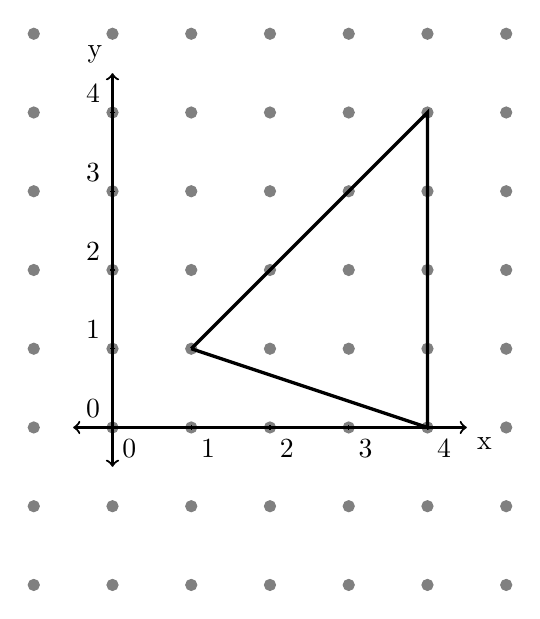
\begin{tikzpicture}
\foreach \x in {-1,0,1,2,3,4,5}
\foreach \y in {-2,-1,0,1,2,3,4,5}
	\filldraw [gray] (\x, \y) circle (2pt);
\draw[thick,<->] (-0.5,0) -- (4.5,0) node[anchor=north west] {x};
\draw[thick,<->] (0,-0.5) -- (0,4.5) node[anchor=south east] {y};
\foreach \x in {0,1,2,3,4}
	\draw (\x cm,1pt) -- (\x cm,-1pt) node[anchor=north west] {$\x$};
\foreach \y in {0,1,2,3,4}
	\draw (1pt,\y cm) -- (-1pt,\y cm) node[anchor=south east] {$\y$};
	
\draw [black, very thick] (1,1) -- (4,0) -- (4,4) -- (1,1);
\end{tikzpicture}
\caption{Graphical depiction of iteration space with dependent $y$ dimension.}\label{triangularIterationSpace2}
\end{subfigure}
\hspace{0.05\columnwidth}
\begin{subfigure}{0.55\columnwidth}
\begin{subfigure}{\columnwidth}
\begin{align}
	1 \leq &x < 5 \\
	(4/3 - x/3) \leq &y \leq x
\end{align}
\caption{Constraint description of iteration space from~\ref{triangularIterationSpace2}.}\label{constraintDescription2}
\end{subfigure}

\vspace{20pt}

\begin{subfigure}{\columnwidth}
\begin{lstlisting}[]
auto x_seg = make_symbolic_segment(1,5);
auto y_seg = make_symbolic_segment(
							(4 - x_seg) / 3, 
							x_seg + 1);
auto segments = make_tuple(x_seg, y_seg);
\end{lstlisting}
\caption{Description of iteration space from~\ref{triangularIterationSpace2} using symbolic segments.}\label{symseg2}
\end{subfigure}
\end{subfigure}
\caption{Two examples of representable triangular iteration spaces.}\label{goodTriangles}
\end{figure}



\begin{figure}
\begin{subfigure}{0.4\columnwidth}
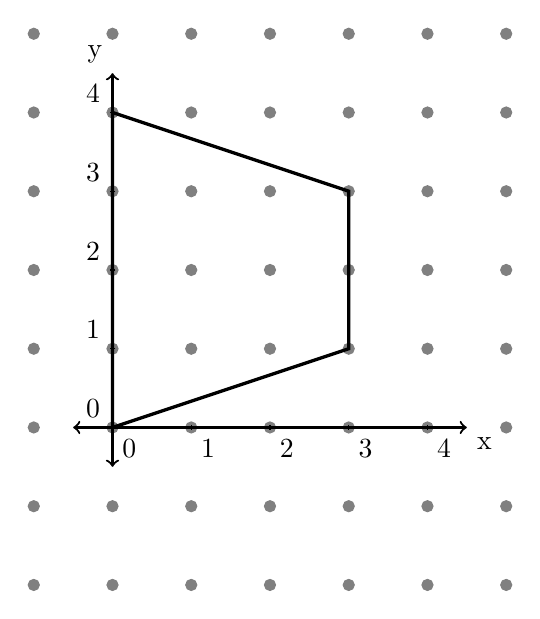
\begin{tikzpicture}
\foreach \x in {-1,0,1,2,3,4,5}
\foreach \y in {-2,-1,0,1,2,3,4,5}
	\filldraw [gray] (\x, \y) circle (2pt);
\draw[thick,<->] (-0.5,0) -- (4.5,0) node[anchor=north west] {x};
\draw[thick,<->] (0,-0.5) -- (0,4.5) node[anchor=south east] {y};
\foreach \x in {0,1,2,3,4}
	\draw (\x cm,1pt) -- (\x cm,-1pt) node[anchor=north west] {$\x$};
\foreach \y in {0,1,2,3,4}
	\draw (1pt,\y cm) -- (-1pt,\y cm) node[anchor=south east] {$\y$};
	
\draw [black, very thick] (0,0) -- (0,4) -- (3,3) -- (3,1) -- (0,0);
\end{tikzpicture}
\caption{Graphical depiction of quadrilateral iteration space with dependent $y$ dimension.}\label{trapezoidIterationSpace1}
\end{subfigure}
\hspace{0.05\columnwidth}
\begin{subfigure}{0.55\columnwidth}
\begin{subfigure}{\columnwidth}
\begin{align}
	0 \leq &x < 4 \\
	x / 3 \leq &y \leq 4 - (x / 3)
\end{align}
\caption{Constraint description of iteration space from~\ref{trapezoidIterationSpace1}}\label{trapezoidConstraint1}
\end{subfigure}

\vspace{20pt}

\begin{subfigure}{\columnwidth}
\begin{lstlisting}[]
auto x_seg = make_symbolic_segment(0,4);
auto y_seg = make_symbolic_segment_inclusive(
							x_seg / 3, 
							4 - (x_seg / 3));
auto segments = make_tuple(x_seg, y_seg);
\end{lstlisting}
\caption{Description of iteration space from~\ref{trapezoidIterationSpace1} using symbolic segments.}\label{trapseg1}
\end{subfigure}
\end{subfigure}
\caption{An example irregular quadrilateral iteration space that can be represented using symbolic segments.}\label{trapezoid1}
\end{figure}



\begin{figure}
\begin{subfigure}{0.5\columnwidth}
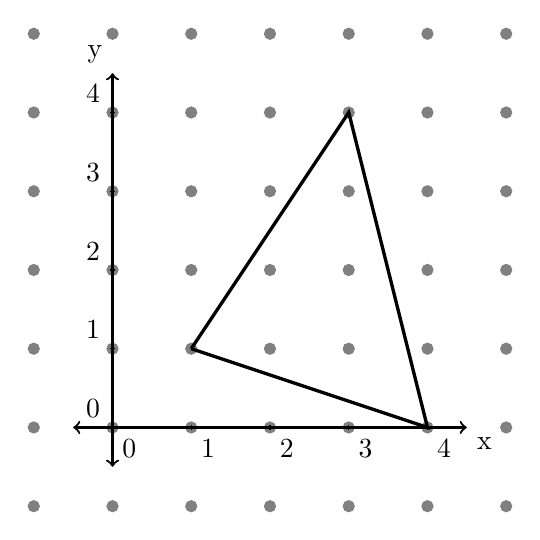
\begin{tikzpicture}
\foreach \x in {-1,0,1,2,3,4,5}
\foreach \y in {-1,0,1,2,3,4,5}
	\filldraw [gray] (\x, \y) circle (2pt);
\draw[thick,<->] (-0.5,0) -- (4.5,0) node[anchor=north west] {x};
\draw[thick,<->] (0,-0.5) -- (0,4.5) node[anchor=south east] {y};
\foreach \x in {0,1,2,3,4}
	\draw (\x cm,1pt) -- (\x cm,-1pt) node[anchor=north west] {$\x$};
\foreach \y in {0,1,2,3,4}
	\draw (1pt,\y cm) -- (-1pt,\y cm) node[anchor=south east] {$\y$};
	
\draw [black, very thick] (1,1) -- (3,4) -- (4,0) -- (1,1);
\end{tikzpicture}
\caption{Nonrepresentable triangular iteration space. $x$ and $y$ dimensions are defined circularly.}\label{triangularIterationSpace3}
\end{subfigure}
\begin{subfigure}{0.5\columnwidth}
\begin{subfigure}{\columnwidth}
\begin{align}
	&y \geq 4/3 - x/3 \\
	&y \leq (3 * x - 1) / 2 \\
	&x \leq 4 - y/4
\end{align}
\caption{Constraint description of iteration space in~\ref{triangularIterationSpace3}}\label{constraintDescription3}
\end{subfigure}

\begin{subfigure}{\columnwidth}
\begin{lstlisting}[caption={C-style loop bounds generated using polyhedral code generator.},label=farkasResult]
for (int x = 1; x <= 4; x += 1) {
	for (int y = -((x + 2) / 3) + 2; 
			 y <= min(-4 * x + 16, x + (x + 1) / 2 - 1); 
			 y += 1) {
		...
	}
}
\end{lstlisting}
\end{subfigure}

\end{subfigure}

\vspace{10pt}

\begin{subfigure}{0.5\columnwidth}
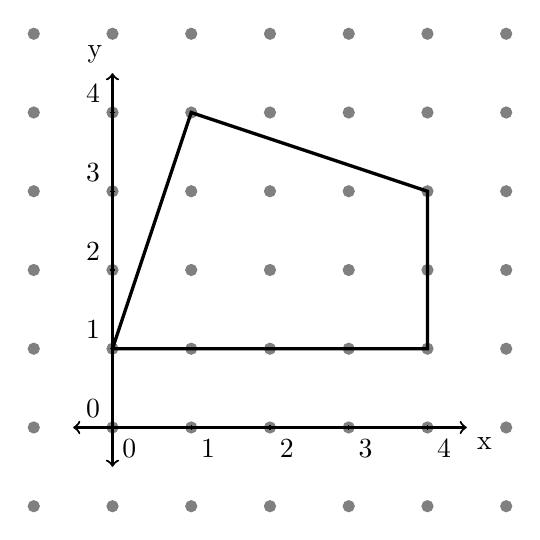
\begin{tikzpicture}
\foreach \x in {-1,0,1,2,3,4,5}
\foreach \y in {-1,0,1,2,3,4,5}
	\filldraw [gray] (\x, \y) circle (2pt);
\draw[thick,<->] (-0.5,0) -- (4.5,0) node[anchor=north west] {x};
\draw[thick,<->] (0,-0.5) -- (0,4.5) node[anchor=south east] {y};
\foreach \x in {0,1,2,3,4}
	\draw (\x cm,1pt) -- (\x cm,-1pt) node[anchor=north west] {$\x$};
\foreach \y in {0,1,2,3,4}
	\draw (1pt,\y cm) -- (-1pt,\y cm) node[anchor=south east] {$\y$};
	
\draw [black, very thick] (0,1) -- (1,4) -- (4,3) -- (4,1) -- (0,1);
\end{tikzpicture}
\caption{Nonrepresentable quadrilateral iteration space. $x$ and $y$ dimensions are defined circularly.}\label{trapezoidIterationSpace2}
\end{subfigure}
\begin{subfigure}{0.5\columnwidth}
\begin{align}
	-1/3 + y/3 \leq &x \leq 4 \\
	1 \leq &y \leq (13-x) / 3
\end{align}
\caption{Constraint description of iteration space in~\ref{trapezoidIterationSpace2}}\label{trapezoidConstraint2}
\end{subfigure}

\caption{Two examples of irregular iteration spaces that cannot be represented using symbolic segments. They are not representable because the dimension bounds are defined circularly.}\label{badShapes}
\end{figure}
%https://compsys-tools.ens-lyon.fr/iscc/index.php

\section{Transforming Data Layouts}

\begin{figure}
\begin{lstlisting}[caption={Changing data layouts for three Views in the \textsc{3mm} benchmark using \FormatDecisions.},
	label={FormatDecisions3MM}]
auto knl1 = make_kernel<KPOL>(segs1, [=](auto i0, auto i1, auto i2) {
	E(i0, i1) += A(i0, i2) * B(i2, i1);
});
auto knl2 = make_kernel<KPOL>(segs2, [=](auto i0, auto i1, auto i2) {
	F(i0, i1) += C(i0, i2) * D(i2, i1);
});
auto knl3 = make_kernel<KPOL>(segs3, [=](auto i0, auto i1, auto i2) {
	G(i0, i1) += E(i0, i2) * F(i2, i1);
});

auto decisions = format_decisions(ref_tuple(B,D,F), knl1, knl2, knl3);

decisions.set_format_for(B, {{1,0}}, knl1); // column-major
decisions.set_format_for(D, {{1,0}}, knl2); // column-major
decisions.set_format_for(F, {{0,1}}, knl2); // row-major
decisions.set_format_for(F, {{1,0}}, knl3); // column-major

// Generate and run the computations with format conversions
auto computation = decisions.generate();
computation();
\end{lstlisting}
\end{figure}

RAJA's existing support for changing data layouts is limited to the point of instantiation.
This work removes that barrier by providing a declarative data optimization system for specifying layout transformations between loops.
By combining user-guided layout specifications with optional automated support, \FormatDecisions{} gives the programmer more control over the optimization of their program.

\subsection{User-Guided Layout Transformations}

Consider the computation in Listing~\ref{SelectionExampleCode}.
Throughout the computation, the data is accessed in different orders.
For example, note the Views \verb.A., \verb.B., and \verb.D..
The order in which \verb.A. is accessed is different from \verb.D. because the argument order in their accesses are different.
In contrast, while \verb.B. and \verb.D. have the same argument order, their access orders are still different because they have different layouts.
Looking at the two references to \verb.F. in kernels two and three, we can see that even access order to the same data can change through a computation.
Because different formats are optimal for different kernels, this creates an opportunity for optimization. 

My approach, shown in action in Listing~\ref{FormatDecisions3MM}, introduces a single user-facing class, appropriately named \verb.FormatDecisions..
Rather than inserting code blocks to change a View's data layout between kernel executions, the user register choices for what format the data should have during different computations. 
Once the user has finished registering their choices, they can launch the supplementary model to identify additional optimizations or immediately generate the loop chain containing the computations and the conversions.

The user registers format decisions with two methods.
The first, \verb.set_format_for()., takes as arguments the View, the desired dimensional ordering, and the kernel or kernels for which the format should be used.
The second method, \verb.set_output_format()., takes a View and a dimensional ordering and ensures the View has that layout after the sequence of computations is done executing.
Lines 13 through 17 of Listing~\ref{FormatDecisions3MM} show four such registered choices.

While \FormatDecisions{} provide a supplementary decision model that can identify additional worthwhile layout changes, its use is not mandatory.
To ``fill-in'' the user's choices with those of the model, the programmer can use the \verb.model(). method.
Because this method uses the symbolic evaluation capabilities provided by RAJALC, it can only be used when the operations are supported for symbolic evaluation.
This means that the kernels cannot make indirect accesses (\verb.a(b(i)).), or call functions within the lambdas that use the iterators.

Regardless of whether the user has used the model or not, 
the complete computation with interspersed format conversions is generated using the \verb.generate(). method.

\subsection{Selecting Decision Semantics}

At first glance, it may seem that a single method for registering format choices would be sufficient. 
Simply provide the View, the computation, and the format to use during that computation.
However, it is often desirable to specify the format the data should be in at the end of the sequence of computations, especially when the sequence is run many times, for example as part of the time step in a simulation code.
A single registering function cannot provide this capability. 

Another important consideration is the semantics of the registered decisions. 
Should the user be registering format conversions or should they be registering the format with the assumption that any necessary conversion is made by the library?
I argue that it should be the latter.
First, registering formats is more declarative, as it does not dictate exactly how or when the data is converted to the desired format.
Second, registering conversions requires specification of both the input and output formats. 
Any conversion can be specified with two format registrations, but no number of conversion registrations can specify the same thing as a single format registration.

With these considerations in mind, I decided on two methods: \verb.set_format_for. and \verb.set_output_format..
When choosing this pair, the shorter \verb.set_format. was considered, but lacks the mnemonic match between the words of the method name and the parameter order. You \textbf{set} the View to \textbf{format} X \textbf{for} computation Y. 
Examples of these methods in use are shown in Listing~\ref{FormatDecisions3MM}.


\section{Automatic Layout Selection}

\FormatDecisions{} supports optional automated layout selection through the \verb.model(). method.
Broadly, the system constructs a search space of possible choices, estimates their costs based on a performance model, and selects the one with the lowest cost.
The problem of automatic layout selection has been formulated as an integer linear programming (ILP) problem by Bixby, Kennedy, and Kremer~\cite{bixby1994automatic}.
The system used within \FormatDecisions{} is based on their formulation, but makes several modifications.
First, instead of using a static cost model, \FormatDecisions{} estimates costs using runtime microbenchmarking.
Second, it uses a modified heuristic for determining the candidate layouts to include in the model.
Finally, \FormatDecisions{} uses a nonlinear integer programming formulation to reduce the number of decision variables, counterintuitively improving solve time (see Section~\ref{sec:modelExperiments}).

This section begins with an overview of the layout selection problem and the prior formulation of Bixby, Kennedy, and Kremer.
It then details the modifications made in \FormatDecisions{}.
It concludes with six experiments that illustrate the effects of different parameters on model solve time, as well as the impact of the switch from a linear to nonlinear optimization problem.

\subsection{The Layout Selection Problem}

Layout selection is a decision problem.
It asks: Given an array and a series of $N$ loop nests accessing the data in $W$ different ways (e.g. \verb.A(i,j)., \verb.A(j,i)., \dots), what data layout should the array have during each loop nest to maximize performance?
Valid answers come as a list of $N+1$ layouts, one to use for each loop nest and one for the array to be in at the end.
For an isolated loop nest with only one kind of access to the array, the optimal answer is usually evident from a visual inspection of the code; the best layout is the one that matches the layout to the access order.
For example, in Listing~\ref{SelectionExampleCode}, \verb.T1. should be in row-major order, while \verb.B. should be in column-major order. 
However, when considering even two loop nests in sequence, the optimal choice is no longer statically evident.
This is because the benefit of using the optimal layout for a loop nest must be weighed against the cost of converting the data from one layout to another.
The challenge is further compounded by architectural differences that can affect both the cost of conversion and which layout will perform optimally.
The difficulty of this comparison lends itself to runtime automation.

Automating the layout selection problem, like many other decision problems, follows a two-step process: generate a set of valid solutions, then search the set for the best one.
Different problems operationalize these two steps in different ways, but a common approach is to model the decision problem as an integer linear programming (ILP) problem.
An ILP problem consists of a set of integer variables representing decision components, linear constraints over those variables representing the relationships between parts of the decision, and a linear objective function representing the costs of making different choices.
The solution to an ILP problem is a mapping of variables to values that satisfies the constraints and minimizes the objective function.
Once the solution to the ILP model has been identified, it can be mapped back to an optimal answer to the original decision problem.

Bixby, Kennedy, and Kremer (BKK) develop such a formulation for the layout selection problem~\cite{bixby1994automatic,kennedy1995automatic,kennedy1998automatic}.
They use a restricted type of ILP problem, known as a 0--1 ILP problem, that only uses binary variables.
Because the variables can only have the values 0 or 1, they can be conceptualized as on-off ``switches.''
Their formulation uses two types of variables: layout switches and remapping switches.
For each loop nest, or ``phase'', there is one layout switch for each possible layout.
Because an array has exactly one layout at a time, one and only one switch can be on for each phase.
Remapping switches represent the layout transformations that occur between phases of the program.
At each remapping point, there is one switch for each possible layout transformation.
As with layouts, only one remapping can occur at a time, so there will be one remapping switch turned on for each remapping point.
Remapping switches are also constrained to match the layout switches.
For example, if the row-major switch is turned on for both the first and second phase, the row-to-column-major remapping switch cannot be turned on.

Using this ILP model, valid solutions to the layout selection problem are represented by constraint-satisfying configurations of the switches.
For a $D$-dimensional array over $N$ loop nests, there are $D!*(N+1)$ such valid solutions, some better than others.
The objective function makes it possible to compare the quality of different solutions, ultimately leading to the best possible choice.
In the BKK formulation, the objective function is a sum of products, with one term for each switch.
Each layout variable is multiplied by a coefficient representing the estimated cost of using that layout for that phase.
Similarly, each remapping variable is multiplied by a coefficient representing the estimated cost of performing that layout transformation.
These cost estimates only contribute to the objective function value when their associated switches are turned on.
The configuration of switches that minimizes the objective function corresponds to a solution to the layout selection problem that should provide the best performance.

The accuracy of a solution relies on the accuracy of the model used to select it.
For the layout selection problem, the most important factor is the accuracy of the cost coefficients.
In the BKK formulation, the cost coefficients are calculated using static performance models based on pre-run training sets using vendor-specific communication libraries~\cite{kremer1996automatic}.
Thus, the quality of their layout selection system is entirely determined by the quality of this performance model.
Because the BKK performance model is static, each new machine requires a new and unique performance model be added to the system.
This limits the system's portability.

The model \FormatDecisions{} uses to solve the layout selection problem is a modified version of the BKK formulation.
There are three key differences.
First, the model is solved at runtime, rather than as part of a programming tool, using microbenchmarking results to inform the cost coefficients (Section~\ref{sec:microbenchmarking}).
Second, the model uses an alternative approach to selecting candidate data layouts (Section~\ref{sec:candidateSelection}).
Third, the model uses a nonlinear objective function (Section~\ref{sec:nonlinearFunc}).

\subsection{Runtime Solving and Microbenchmarking}\label{sec:microbenchmarking}

Where the BKK model is incorporated into a static, pre-compilation programming tool, \FormatDecisions{} solves the layout selection problem at runtime.
Because the model is solved at runtime, \FormatDecisions{} gains two sources of information not present in the BKK formulation.
First, \FormatDecisions{} has access to program parameters, like loop bounds and array sizes that are not available to the static BKK system.
Second, \FormatDecisions{} is able to more accurately estimate the costs of different data layouts by incorporating microbenchmarking results into the objective function.
These microbenchmarks are run as part of the program's execution, so they will be tuned to the architecture, system, and even the specific node on which the program runs.
While runtime solving can incorporate previously unavailable information, it comes with runtime overhead.
This runtime overhead must be outweighed by the performance improvement of the layout optimization, so the smaller the model, the better.
The second and third modifications to the BKK model are motivated by this need for a quick model, but first I turn to the runtime microbenchmarking.

\FormatDecisions{} uses runtime microbenchmarking to estimate the costs of using and converting among the candidate layouts. 
For different data accesses, a streaming copy with the same access pattern is timed at runtime.
The results of the microbenchmarking are incorporated into the model as the coefficients on the decision variables in the objective function.
The approach considers two types of costs: use costs and conversion costs.
Use costs represent the anticipated execution time associated with accesses to the data during the computation itself.
Conversion costs represent the anticipated execution time associated with converting from one format to another in between phases.
They use different approaches to determine their contributions to the objective function.

Use cost determination is access-based and proceeds through each kernel (phase) in the loop chain.
First, the kernel is symbolically evaluated and accesses to the View being modeled are isolated.
For each access, one term will be added for each candidate layout, estimating the cost of making that access with the candidate layout.
This estimate is the product of the microbenchmarking time and the number of loop iterations that make the access.
The microbenchmark is selected to match the traversal order of the access using that layout.

Collapsing the access, schedule, and candidate layout into the traversal order allows microbenchmark results to be reused for different variables. 
For example, for a constant schedule, the access \verb.A(i,j). in row-major layout has the same traversal order as the access \verb.A(j,i). in column-major layout.
Thus, their performance can be modeled with the same microbenchmark result. 
By reusing a single timing result for multiple decision variables, the overall time necessary to run the decision model is reduced.

The microbenchmarking results from the use cost estimation can be reused further to estimate conversions costs.
The key insight here is that a conversion from one format to another is itself a computation and can be modeled as such.
The conversion computation makes one access to data in the source layout, and one access to data in the destination layout. 
Thus, the conversion cost is the sum of these two accesses.

\begin{comment}
\begin{lstlisting}[caption={Algorithm for generating the objective function's use cost terms.}]
SumExpression estimate_use_costs(knls, modeledView, candidateLayouts) {
	SumExpression useCosts();

	for knl in knls:
	  for access in knl.evaluate_symbolically():
		  if access.view == modeledView:
			  for layout in candidateLayouts:
				  traversalOrder = calc_traversal_order(knl.schedule, access.argOrder, layout);
					accessTime = time_microbenchmark(traversalOrder)
					costCoefficient = accessTime * knl.numIterations;

					decisionVar = LayoutVariable(knl, layout);
					costTerm = MultExpression(costCoefficient, decisionVar);
					useCosts.add(costTerm);
	
	return useCosts;
}
\end{lstlisting}

\begin{lstlisting}[caption={Algorithm for generating the objective function's conversion cost terms.}]
SumExpression estimateConversionCosts(knls, modeledView, candidateLayouts) {
	SumExpression conversionCosts();

	for inputLayout in candidateLayouts:
		for outputLayout in candidateLayouts:
			readTime = timeMicrobenchmark(defaultSchedule, defaultArgOrder, inputLayout);
			writeTime= timeMicrobenchmark(defaultSchedule, defaultArgOrder, outputLayout);
			costCoefficient = (readTime + writeTime) * modeledView.size();

			for inPhase in 0 to numKnls:
				outPhase = inPhase + 1;
				inVar = LayoutVariable(inPhase, inputLayout);
				outVar = LayoutVariable(outPhase, outputLayout);
				costTerm = MultExpression(inVar, outVar, costCoefficient);
				conversionCosts.add(costTerm);
	
	return conversionCosts;
}
\end{lstlisting}

\begin{lstlisting}[caption={Algorithm for microbenchmark timing. Implementation is shown for two-dimensional case. Actual implementation uses template metaprogramming to generalize the dimensionality.}]
SumExpression timeMicrobenchmark(scheduleOrder, argumentOrder, layoutOrder) {
	static std::map<...> cache; // reuse results from previous microbenchmarking

  normalizedLayoutOrder = normalize(scheduleOrder, argumentOrder, layoutOrder);

	if (cache[normalizedLayoutOrder] != 0) {
		return cache[normalizedLayoutOrder];
	}

	idx_t n = pow(modelProblemSize, 1/2.0);

	//allocate memory and create Views
	double* data1 = new double[modelProblemSize];
	double* data2 = new double[modelProblemSize];
	View2D arr1(data1, normalizedLayoutOrder);
	View2D arr2(data2, normalizedLayoutOrder);

	//fill Views
	for(int i = 0; i < modelProblemSize; i++) {
		data1[i] = std::rand();
		data2[i] = std::rand();
	}

	using Policy = NestingPolicy<2>;

	auto lam = [=](auto i, auto j) {
	  arr2(i,j) = arr1(i,j);
	};
	auto segments = make_tuple(RangeSegment(0,n), RangeSegment(0,n));

	auto knl = make_kernel<Policy>(lam, segments);

	startTimer();
	knl();
	elapsed = stopTimer();

	cache[normalizedLayoutOrder] = elapsed;
	return cache[normalizedLayoutOrder];
}
\end{lstlisting}

\end{comment}
Because the cost of conversion does not change based on the number of accesses to the data, these terms can be generated without reference to their surrounding computations.
Furthermore, they can be constructed while reusing the microbenchmarking results from the use cost estimation.
This is because a conversion from one layout to another can naturally be viewed as a kernel with two accesses: one access to data in the source layout and one to data in the destination layout.
Thus, the cost coefficient becomes the size of the array multiplied by the sum of the two access estimates.


\subsection{Candidate Layout Selection}\label{sec:candidateSelection}

The second modification refines how the model determines which layouts to include as candidates for selection.
The BKK formulation does not detail how their model makes this choice, but only discusses two-dimensional data, where there are only two possible orderings.
For higher-dimensional data, a simple option is to fully enumerate the possible layouts.
For two dimensional data, this gives two options; for three dimensional, six; for four, 24.
As the dimensionality increases, the number of layouts increases dramatically, and with it the modeling time.
Thus, an alternative formulation for selecting candidate layouts is needed.

Rather than using all $D!$ possible layouts, \FormatDecisions{} generates its set of candidate layouts using a seed set and a generating function.
The seed set is a small set of layouts which is expanded to a larger, final set of candidates using the generating function.
The seed set includes the original layout of the data, any layouts the user provides as part of registered decisions, and any layouts that \FormatDecisions{} calculates to match the access orders within the loop nests.
The generating function takes this set of seed layouts and generates the final set of candidates.
The generating function is user-configurable, but the default function is repeated rotation.
Rotating a layout means shifting each dimension to the right and moving the rightmost index to the leftmost position.
For example, repeatedly rotating the layout $(0,1,2)$ produces the layout $(2,0,1)$, then $(1,2,0)$, and finally $(0,1,2)$. 
Using this scheme, the number of candidate layouts is reduced from $O(D!)$ to $O(D)$, further reducing modeling time.

Repeated rotation was selected as the generating function for a confluence of reasons.
First, the generating function needs to generate options that are not present in the original set of options.
This excludes the identity transformation.
Second, different architectures perform better with different stride lengths.
While a CPU will do well with low-stride accesses, a GPU will perform better with large-stride accesses.
Because repeated rotation generates options where every dimension shows up once in each position, it is guaranteed to produce a wide range of stride lengths.
Finally, rotation is a staple, comprehensible transformation with transparent behavior.
This makes for easier reasoning about the model's decisions.
While it is possible that rotation will not surface the maximally performant layout for higher-dimensional data, the layout options it produce are a launching point for further experimentation.
Furthermore, user can supply an arbitrary generating function as long as it maps containers of layout permutations to containers of layout permutations.

\subsection{Nonlinear Objective Function}\label{sec:nonlinearFunc}

Minimizing solve time also led to the third key difference between the BKK formulation and the \FormatDecisions{} formulation: the use of a nonlinear objective function.
Execution time attributable to the ILP model comes from two sources: problem initialization (setup), and objective function minimization (solve).
The setup phase initializes the objects for the space of constrained decision variables and the objective function.
The more decision variables and constraints, the longer the setup phase.
The solve phase applies the objective function to the decision space and identifies the minimum point.
This too scales with the number of decision variables and constraints.
Using a nonlinear objective function can eliminate the majority of the decision variables in the problem.
While search time per decision variable increases with this scheme, the overall model time decreases significantly.

The nonlinear formulation reduces modeling time by completely eliminating remapping variables.
Recall that the BKK formulation uses two types of decision variables in its ILP model: layout variables and remapping variables.
Further, recall that the model constraints ensure the remapping variables between two phases are matched to the layout variables for those phases.
Given these constraints, the remapping variables are completely determined by the layout variables; 
if we know the values of the layout variables, we can always reconstruct the values of the remapping variables.
So then what is the purpose of the remapping variables? 
Simply, it is to incorporate the \textit{cost of remapping} into the linear objective function.
Because there are remapping variables for each pair of layouts, a model with $O(N)$ layout variables will need $O(N^2)$ remapping variables.
As a result, these faux variables end up dominating the entire model and bloat execution time.

Remapping variables are eliminated using a replacement scheme. 
Because their values are fully determined by the layout variables, remapping variables in the decision space and constraints containing them can be removed without incident.
This only leaves the terms containing remapping variables in the objective function.
These are replaced with equivalent terms that encode the removed constraints.
A remapping variable can only be switched on when the layout variables corresponding to its input and output are switched on.
This is a familiar operator: logical and --- or in the realm of boolean algebra, multiplication.
For example, all occurances of the remapping variable representing converting from row- to column-major between phases 1 and 2, $remap_{rowmjr \rightarrow colmjr}^{phase1 \rightarrow phase2}$, would be replaced by the product $layout_{rowmjr}^{phase1} * layout_{colmjr}^{phase2}$.
Thus, a replacement scheme can replace remapping variables in the objective function with products of layout variable.
This produces a nonlinear function, as it multiplies variables by other variables, but reduces the number of decision variables in the problem by a square factor.

\subsection{An Example Selection Problem}
\todo{more hand holding in this section}

An demonstration of the layout selection problem and the approach to solve it is instructive.
Consider the loop chain in Listing~\ref{SelectionExampleCode}, which calculates a series of matrix multiplications.
The layout selection problem in this subsection will target the \verb.A. View.
We construct the constrained decision space, then use microbenchmarking to construct the objective function.

The decision space construction starts with the selection of the candidate layout $L$.
For two-dimensional problems, the two candidates are row-major and column-major.
Within the system, these are represented as dimensional orderings--$(0,1)$ and $(1,0)$--but for clarity's sake, we use their names here: $L=\{row,col\}$.

Once the candidate layouts have been identified, we can create the layout decision variables.
For each phase of the computation, including the input and ouput phases, there is one variable for each layout.
The subscript indicates the layout while the superscript indicates the phase. 
The 0 phase represents the input layout, while the $N+1$ phase represents the output layout.
For example, the $k_{col}^{3}$ variable indicates whether or not the array will use column-major order during the third phase (\verb.knl3).
Thus, the full list of layout variables is: $[k_{row}^{0}, k_{col}^{0}, k_{row}^{1}, k_{col}^{1},k_{row}^{2}, k_{col}^{2},k_{row}^{3}, k_{col}^{3},k_{row}^{4}, k_{col}^{4}]$.

The last step in creating the constrained decision space is the constraint expression. 
First, variables are constrained to be either zero or one. 
Thus, for each decision variable $k$, we add the constraint $0 \leq k \leq 1$.
Next, for each phase, exactly one layout will be selected. 
Thus, for each phase $i$, we add the constraint $\sum_{\ell \in L} k_\ell^{i} \ \ = 1$.
Optionally, a constraint can be added to match the input and output format.
In this circumstance, for each candidate layout $\ell$, we add $k_\ell^{0} = k_\ell^{N+1}$.
Finally, additional constraints are added based on decisions registered by the user, setting the appropriate variable to 1.

Constructing the objective function begins with estimating the cost of accesses to the modeled View.
Starting with the first kernel, symbolic evaluation identifies one access, \verb.A(i,k)..
This access will contribute terms for the decision variables $k_{row}^1$ and $k_{col}^1$, one for each possible layout for \verb.A..
Here, the timing function shown in Listing~\ref{MicrobenchmarkingCode} is run for row-major and column-major layouts.
Because this is the first access being considered, small streaming benchmarks using each layout are executed and timed. 
For this example, assume the row-major layout return a time of 200, and the column-major layout returned a time of 400.
These results are fed into the performance model as the coefficients of terms in the objective function.
For each of the decision variables that this access contributes a term for, the model multiplies the timing result by the number of iterations in which the access appears. 
The timing result where the modeled data accesses with the same pattern is selected.
So for the decision variable $k_{row}^1$, the model will add the term $200 * 1000000 * k_{row}^1$, and for $k_{col}^1$ will add $400 * 1000000 * k_{col}^1$.

In the next kernel, symbolic evaluation identifies another access: \verb.A(k,j)..
Note that with this access, the order of the iterators is reversed. 
This means that the row-major timing result is used as the coefficient for the column-major layout, and vice versa.
Thus, the model will add the terms $200 * 1000000 * k_{col}^2$ and $400 * 1000000 * k_{row}^2$.
The modeling result is always selected to match the data access pattern that the data would have for that layout.
The third kernel proceeds similarly with the access \verb.A(k,i)..
The model will add the terms $200 * 1000000 * k_{col}^3$ and $400 * 1000000 * k_{row}^3$.

Next, the model adds terms to represent the cost of converting between layouts. 
For each pair of different layouts and consecutive kernels (including the input and output placeholders), one term is added representing the reads and writes required to convert layouts.
For example, to represent the cost of converting from column-major to row-major between kernels 2 and 3, the model will add $400 * 10000 * k_{col}^2 * k_{row}^3$ to represent the read of the column-major data and $200 * 10000 * k_{col}^2 * k_{row}^3$ to represent the write to the row-major data.
Both decision variables are part of the term to ensure the cost is only contributed when those layouts are selected.

Once the objective function is generated, it is applied to the space of layout choices, and the choice with the smallest score is identified.
This choice represents the layout transformations that the model predicts will lead to the fastest execution time.
For this example, the model will choose row-major for the first computation and column-major for the second and third.

\begin{figure}
\begin{lstlisting}[caption={Example loop chain. The selection problem targets the \texttt{A} array. Code is shown using standard C++ for loops rather than RAJA kernels for the reader's familiarity.},label=SelectionExampleCode]
int N = 100;
//knl1
for (i = 0; i < N; i++) {
	for(j = 0; j < N; j++) {
		for(k = 0; k < N; k++) {
			T1(i,j) += A(i,k) * B(k,j);
		}
	}
}
//knl2
for (i = 0; i < N; i++) {
	for(j = 0; j < N; j++) {
		for(k = 0; k < N; k++) {
			T2(i,j) += T1(i,k) * A(k,j);
		}
	}
}
//knl3
for (i = 0; i < N; i++) {
	for(j = 0; j < N; j++) {
		for(k = 0; k < N; k++) {
			T3(i,j) += A(k,i) * T2(k,j);
		}
	}
}

\end{lstlisting}
\end{figure}

\begin{figure}
	\begin{lstlisting}[caption={Microbenchmarking function for determining objective function cost coefficients. Code is shown for two-dimensional case for clarity. Note that the size of the data in the timed kernel does not change based on the size of the loops being modeled.},label=MicrobenchmarkingCode]
	size_t modelLayoutCost(Layout<2> l) {
		static std::map<Layout<2>, size_t> cacheMap;
		if (cacheMap[l] != 0) return cacheMap[l];

		int sideLength = sqrt(modelDataSize);
		View2D v1(new double[sideLength*sideLength], l);
		View2D v2(new double[sideLength*sideLength], l);

		// ... fill v1 and v2 with random data

		auto iterDim = RangeSegment(0,sideLength);
		auto iterationSpace = make_tuple(iterDim, iterDim);

		auto startTime = currentTime(); // millisecond resolution
		kernel<Pol2D>((iterSpace, [&](auto i, auto j) {
			v2(i,j) = v1(i,j);
		});
		auto stopTime = currentTime()
		auto elapsedTime = stopTime - startTime;

		cacheMap[l] = elapsedTime;
		return cacheMap[l];
	}
	
	\end{lstlisting}
\end{figure}

\subsection{Six Parameters, Six Experiments}\label{sec:modelExperiments}

To illustrate the workings of the layout selection model, I evaluate its use for six synthetic programs that each vary one parameter: loop count, loop depth, memory footprint, access count, user constraint count, or data dimensionality.
Results are reported for two versions of the model.
The ``Linear Model'' panels use the BKK formulation of the optimization problem.
This means that it uses remapping variables, a linear objective function, and exhaustively enumerates the candidate layouts.
The ``Nonlinear Model'' panels use the optimized \FormatDecisions{} formulation.
This means that it does not use remapping variables, uses a nonlinear objective function, and uses the rotation heuristic for identifying candidate layouts.
For each experiment, I break the modeling time into the time spent modeling different access patterns, the time spent initializing the decision space and objective function, and the time spent identifying the optimal point within the decision space. 
Overall, data dimensionality, loop count, and user constraint count have the most impact on the modeling time.
Loop depth and memory footprint have no impact on modeling time, while access count has a small impact.

\begin{figure}
	\includegraphics[width=0.5\columnwidth]{DataDimensionality.pdf}
	\caption{Changes in modeling time for data with different numbers of dimensions.}\label{DataDimensionality}
\end{figure}
The first parameter is the dimensionality of the data, varying in Figure~\ref{DataDimensionality} from two to six, the maximum dimensionality found in a production code (QCD).
The hypothesis is that the modeling time for the heuristic-driven model will increase linearly with the number of dimensions.
\todo{indicate why this hypothesis makes sense}
This hypothesis is partially supported by the results.
Without reducing the set of candidate layout using the rotation heuristic, the execution reaches timeout before completing for four, five, and six dimensions.
For the version using the rotation heuristic, the solve time scales linearly with the dimensionality because the number of decision variables increases linearly with the dimensionality.
\todo{this part of the paragraph is not clear}
The cost estimation time scales faster than linearly, likely because of the dual increases in the number of layouts to model and the number of operations required to calculate the memory offset. 
This would also explain the large jump in cost estimation time between three and four dimensions, as the compiler may not be performing strength reduction on the incrementing for higher dimensional data.

\begin{figure}
\includegraphics[width=0.5\columnwidth]{LoopCount.pdf}
\caption{Changes in modeling time for different loop chain lengths.}\label{LoopCount}
\end{figure}
The next experiment, shown in Figure~\ref{LoopCount}, shows the modeling time for loop chains with between one and eight loop nests.
For this experiment, all loop nests are three-dimensional and make three accesses to two-dimensional arrays of $100\times100$ doubles. 
This size was selected to comfortably fit all data within cache.
No user constraints are added.
Because each new loop nest multiplies the number of possible paths by the number of candidates, the expected behavior is an exponential growth in solve time, which the results supports.
This experiment illustrates the execution time savings of eliminating the remapping variables from the model.
Using the linear model, because there are so many decision variables in the model, the majority of modeling time is spent in setup with as few as four loop nests (57\%).
Overall, the nonlinear model is between $1.29\times$ and $2.63\times$ faster than the linear model in this experiment.

\begin{figure}
	\includegraphics[width=0.5\columnwidth]{NestDepth.pdf}
	\caption{(Lack of) Changes in modeling time for different depths of loop nests.}\label{NestDepth}
\end{figure}
The third experiment, shown in Figure~\ref{NestDepth}, shows the modeling time for loop chains where loop nest depth ranges from two to four.
Here, the loop chain contains three loop nests, and all other parameters are the same as the first experiment.
Because the performance model is data-oriented rather than loop oriented, meaning it seeks to model the performance of each access in the loop rather than the loop as a whole, the hypothesis is that modeling time will remain constant across different nest depths.
The results support this hypothesis.

\begin{figure}
\includegraphics[width=0.5\columnwidth]{Footprint.pdf}
\caption{(Lack of) Changes in modeling time for different memory footprints.}\label{Footprint}
\end{figure}
The fourth experiment varies the size of the arrays accessed by the loop chain, shown in Figure~\ref{Footprint}.
The data sizes were selected to fill multiples of different levels of the evaluation machine's memory hierarchy, with a combination of half-filled, fully filled, or doubly-filled for each of L1, L2, and L3 cache.
These sizes were chosen because they exercise different parts of the memory hierarchy.
See Section~\ref{fillingSizesCalculation} for discussion of how these values are calculated.
Because the model only uses data sizes as coefficients in the model, the modeling times should remain the same as the memory footprint increases.
Aside from small fluctuations, the results support this hypothesis.


\begin{figure}
	\includegraphics[width=0.5\columnwidth]{AccessCount.pdf}
	\caption{Changes in modeling time for different numbers of data accesses.}\label{AccessCount}
\end{figure}
Next is the number of accesses made to the data within the loop body.
Because modeling results are reused where possible, more accesses should not lead to more cost estimation time. 
However, it could lead to slightly higher solve times, as the objective function adds new terms for each access.
The results for this experiment are somewhat unexpected, as cost estimation time scales with the access count.
This is likely due to cost of accessing the cache holding prior estimation results, as the cost estimation increase per additional access is much smaller than the cost of modeling a single access.

\begin{figure}
	\includegraphics[width=0.5\columnwidth]{ConstraintCount.pdf}
	\caption{Changes in modeling time for different numbers of user-provided layout decisions.}\label{ConstraintCount}
\end{figure}

The final parameter is the number of layout decisions the user provides. 
Each additional layout decision adds one constraint, reducing the number of valid configurations. 
This should lead to a reduction in solving time, as there are fewer points to evaluate.
The results support this hypothesis.

\section{Production System}

This section outlines a potential production system based on \FormatDecisions{} that uses representative training runs to entirely offload the overhead of running the decision model.
The production version would use a single feature not present in the prototype: decision I/O.
Specifically, to use the model results from a training run during a later production run, the system would need to be able to write out and read back in the model's layout decisions to persistent files 
This is not a completely trivial feature, but it is not a significant challenge, and I will return to it after outlining the system's function.

The production system would be run in one of two modes.
In the first mode, meant to be run with smaller but representative inputs, the system runs the decision model for each loop chain it encounters, writing the final, comprehensive layout choices to file.
In the second mode, meant to be used on the full production inputs, the system uses the layout choices produced by the training run.
Because the training run writes the full set of layout decisions for each loop chain, no modeling is necessary and the loop chains can be executed immediately.

Of course, it is not always possible to exercise all code paths with a single training run. 
For this circumstance, I propose a hybrid ``learning'' mode.
Meant to be run with full production inputs, it uses previous layout decision files when available and runs decision models for newly encountered loop chains.
Like the training mode, it writes the decisions to file, so that later runs can reuse the results.
With this scheme, newly encountered code paths will incur modeling costs for a single run, but not thereafter.

Returning to the problem of decision I/O, the key insight is that each \FormatDecisions{} object has a unique type in C++.
This is because its type contains the types of all the kernels within it, in the same way that the \verb.int. type is part of a \verb.std::vector<int>. type.
Two \FormatDecisions{} objects created from different kernels, or even from the same kernels in a different order, will have different types, much like a \verb.std::map<int, double>. object is a different type from a \verb.std::map<double, int>..
Thus, the decisions can be indexed by hashing the type of the \FormatDecisions{} object with which the decisions are associated.
Specifically, this can be achieved using C++ \verb.typeid. operator and the \verb.name. method on the resulting \verb.type_info. object.
This would ensure that decisions for a GPU execution are not used for a CPU execution, as the \FormatDecisions{} object types reflect the execution policy types of their constituent kernels.


\section{RAJAPerf Benchmark Evaluation}

This evaluation measures two features: model choice accuracy and system overhead.
Model choice accuracy refers to the accuracy of the runtime performance model by comparing the model decisions against those made by a heuristic-based hand-tuned variant.
This also includes the performance impacts of the model choosing different layouts.
System overhead refers to the runtime overhead from using the \FormatDecisions{} system.
I report two sources of overhead here: ILP overhead from setting up and solving the ILP problem and overhead from the layout selection abstractions.
Runtime microbenchmarking is included in the ILP overhead measurement.
\todo{give the punchline: what was the result}

\subsection{Experimental Design}

I evaluate the \FormatDecisions{} system using six benchmark kernels from the Polybench~\cite{pouchet2012polybench} benchmark suite: \textsc{2mm}, \textsc{3mm} \textsc{correlation}, \textsc{covariance}, \textsc{doitgen}, and \textsc{symm}.
\textsc{2mm} solves the matrix expression $A*B*C$ using two matrix multiplications. 
First, it computes $A*B$ and stores the results in a temporary array.
Then this temporary result is multiplied by $C$.
\textsc{3mm} solves a similar matrix expression $A*B*C*D$ using three matrix multiplications.
It computes $A*B$, then $C*D$, then multiplies the results.
\textsc{correlation} and \textsc{covariance}, as the names suggest, calculate the correlation and covariance matrix for the input data. 
\textsc{correlation} has four loop nests and \textsc{covariance} has three.
\textsc{doitgen} is a multiresolution analysis kernel while \textsc{symm} computes a symmetric matrix-multiplication.
These kernels, especially the matrix multiplication kernels, are ubiquitous computations.
They appear as building blocks across domains, found anywhere with linear algebra or statistics.

Each benchmark has four implemented variants. 
The baseline variant, ``RAJALC'', is implemented using the computation objects described in Chapter 2 and does not apply any layout transformations.
The second variant, ``Hand Tuned'', adds hueristic-based layout transformations \textit{without} using \FormatDecisions{}.
Data layouts are selected to match the access patterns of each computation, without attempting to estimate the tradeoff between conversion cost and performance improvement.
The third variant, ``Model Run'', uses the fully automatic \FormatDecisions{} system to select and apply layout transformations.
The only layout information provided to the model are the output formats for the data.
The fourth variant, ``Model Skipped'', uses the \FormatDecisions{} interface to fully specify the layout transformations given by the performance model, but uses the results of a previous model run.
Thus, this variant does not include overhead from running the performance model.
The difference between the execution times of the ``Hand Tuned'' and ``Model Skipped'' variants is the abstraction overhead, while the difference between the ``Model Skipped'' and ``Model Run'' variants is the ILP overhead.


\subsection{Evaluation Machine Characteristics}
\label{fillingSizesCalculation}
I evaluate application performance on two machines: Lassen and Quartz.
All performance results are collected from single-node runs.
Lassen nodes use two 22-core 3.45GHz IBM Power9 CPUs.
However, a slow inter-socket connection is known to affect execution time consistency when the entire node is used by a single shared-memory program.
The conventional wisdom for Lassen is to treat each processor as its own node, so I run with 22 threads on a single processor.
Quartz nodes each have two 18-core 2.1GHz Intel Xeon E5--2695  CPUs.
Quartz runs in this chapter use a full 36 threads over both processors on the node.
Table~\ref{machineDetails} details the memory hierarchies for both machines.

\begin{table}[t]
	\centering
\begin{tabular}{|c|c|c|c|c|}
\hline
\textbf{Machine Name} & \textbf{L1 Cache} & \textbf{L2 Cache} & \textbf{L3 Cache} & \textbf{RAM} \\
\hline 
Lassen & 704KB & 16896KB & 120MB & 128GB \\ % https://hpc.llnl.gov/documentation/tutorials/using-lc-s-sierra-systems#POWER9
\hline
Quartz & 1152KB & 9216KB & 90MB & 128GB \\ 
\hline
\end{tabular}
\caption{Evaluation machine memory hierarchy characteristics. Cache sizes are given as total sizes for the the evaluation configuration.}\label{machineDetails}
\end{table}
%512*22 + 512*11 = 16896KB %lassen L2
%256*36 = 9216KB %quartz L2
%120MB %lassen L3
%45*2 = 90MB % quartz L3
%128GB % lassen RAM
%128GB % quartz RAM

For each benchmark, I run with six problem sizes on each machine. 
Each problem size half fills, fully fills, or doubly fills either L1 or L2 cache.
While I had attempted to run with sizes that fill L3 cache as well, preliminary executions timed out their node allocations before completing.
This is because the amount of computation scales faster than the amount of data ($N^3$ vs $N^2$).


The sizes for each benchmark are shown in Table~\ref{fillingSizes}.
To calculate these sizes, I use the array counts for the benchmark to construct a polynomial, the solution to which is the dimensional extent that fills a store of a particular size.
For example, the \textsc{covariance} benchmark has one 1D and two 2D arrays. 
To calculate the problem size that fills 704KB (Lassen L3 cache), which holds 60,000,000 doubles, we can construct the polynomial $2x^2 + x^1 = 60000000$.
The positive solution to this equation is the side length that will completely fill Lassen's L3 cache.
Because side lengths must be positive integers, I round down.

\begin{table}
	\centering
	\begin{tabular}{|c|c||c|c|c|c|c|c|}
		\hline
		\multicolumn{2}{|c|}{Benchmark} & SYMM & 2MM & 3MM & CORR & COV & DOITGEN \\ \hline
		\multicolumn{2}{|c|}{Dim Counts} & [0, 3] & [0, 5] & [0, 7] & [2, 2] & [1, 2] & [1, 1, 1] \\ \hline
	\hline
	Size Name & Data Size &   &   &   &   &   &   \\ \hline
	Lassen L1, .5x & 352KB & 242 & 187 & 158 & 296 & 296 & 55 \\ \hline
	Lassen L1, 1x & 704KB & 342 & 265 & 224 & 419 & 419 & 70 \\ \hline
	Lassen L1, 2x & 1408KB & 484 & 375 & 317 & 592 & 593 & 88 \\ \hline
	Lassen L2, .5x & 8448KB & 1186 & 919 & 776 & 1452 & 1453 & 161 \\ \hline
	Lassen L2, 1x & 16896KB & 1678 & 1299 & 1098 & 2054 & 2054 & 203 \\ \hline
	Lassen L2, 2x & 33792KB & 2373 & 1838 & 1553 & 2906 & 2906 & 256 \\ \hline
	Quartz L1, .5x & 576KB & 309 & 240 & 202 & 378 & 379 & 65 \\ \hline
	Quartz L1, 1x & 1152KB & 438 & 339 & 286 & 536 & 536 & 82 \\ \hline
	Quartz L1, 2x & 2304KB & 619 & 480 & 405 & 758 & 758 & 104 \\ \hline
	Quartz L2, .5x & 4608KB & 876 & 678 & 573 & 1072 & 1073 & 131 \\ \hline
	Quartz L2, 1x & 9216KB & 1239 & 960 & 811 & 1517 & 1517 & 166 \\ \hline
	Quartz L2, 2x & 18432KB & 1752 & 1357 & 1147 & 2146 & 2146 & 209 \\ \hline	
\end{tabular}	
\caption{Breakdown of benchmark data use and filling side lengths for different store sizes. The Data Dim Counts row indicates the number of arrays of different dimensionalities used in the benchmark. For example, [1, 2] means the benchmark uses a single 1D array and two 2D arrays. Filling side lengths are calculated by solving polynomials.}\label{fillingSizes}
\end{table}


\subsection{Results}
\begin{figure}
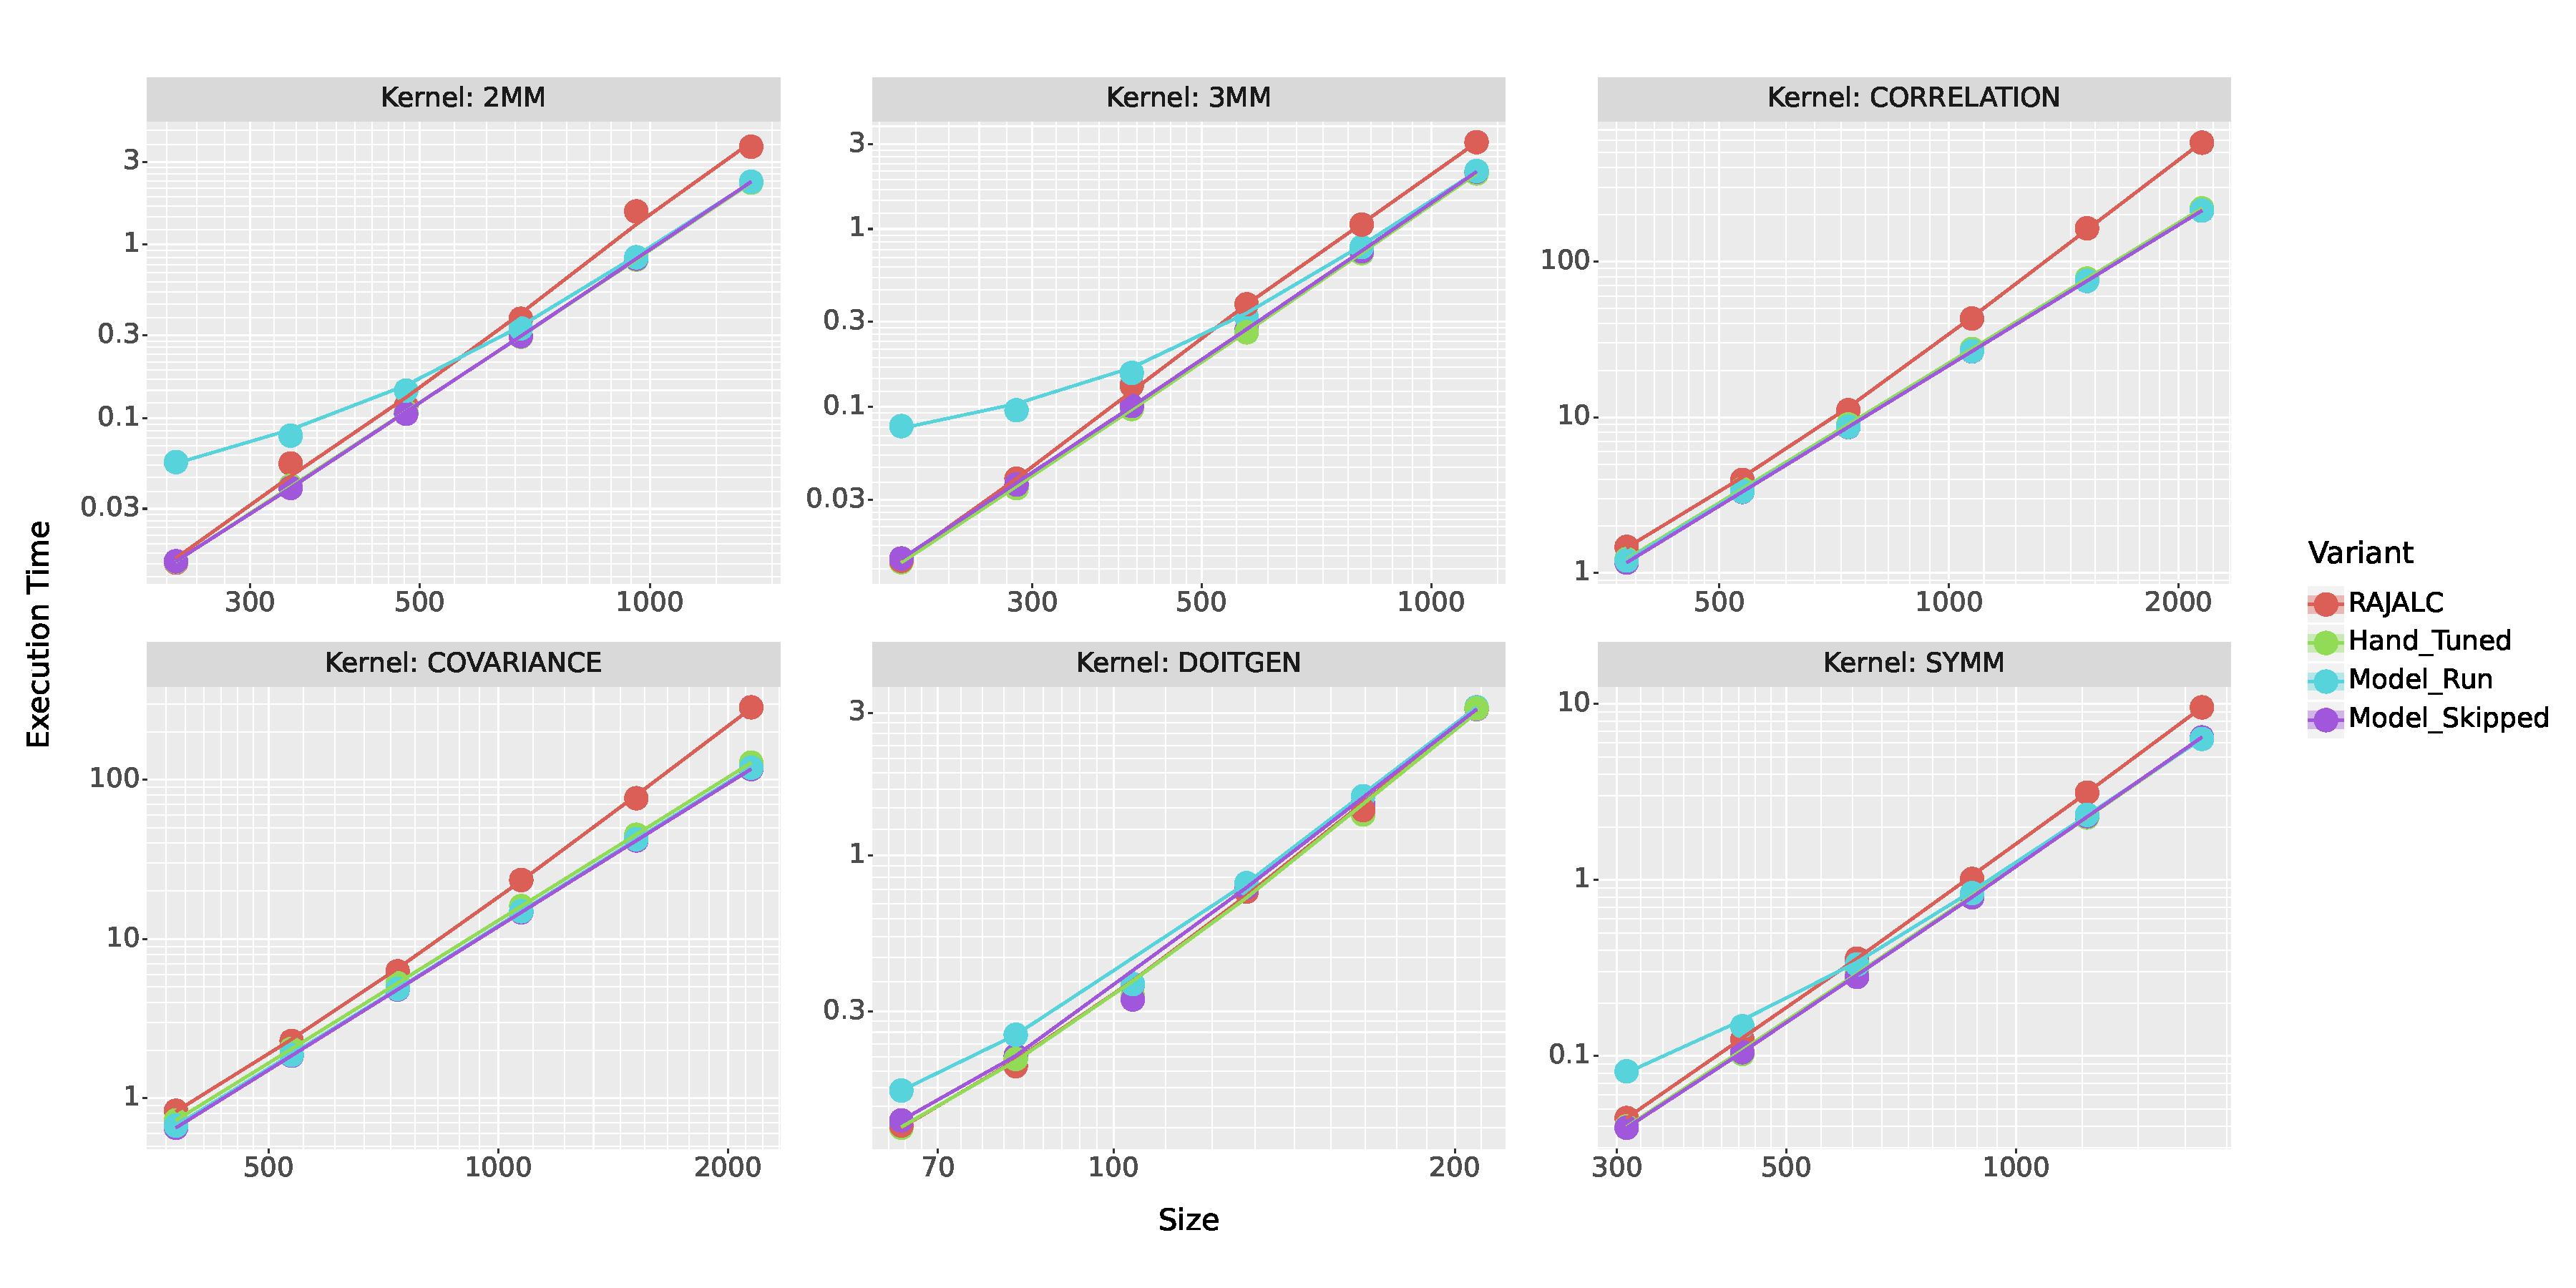
\includegraphics[width=\columnwidth]{quartz_speedups.pdf}
\caption{Execution times for evaluation on the Quartz system. Both axes are log-scale. Lower is better.}
\label{quartzSpeedups}
\end{figure}

\begin{figure}
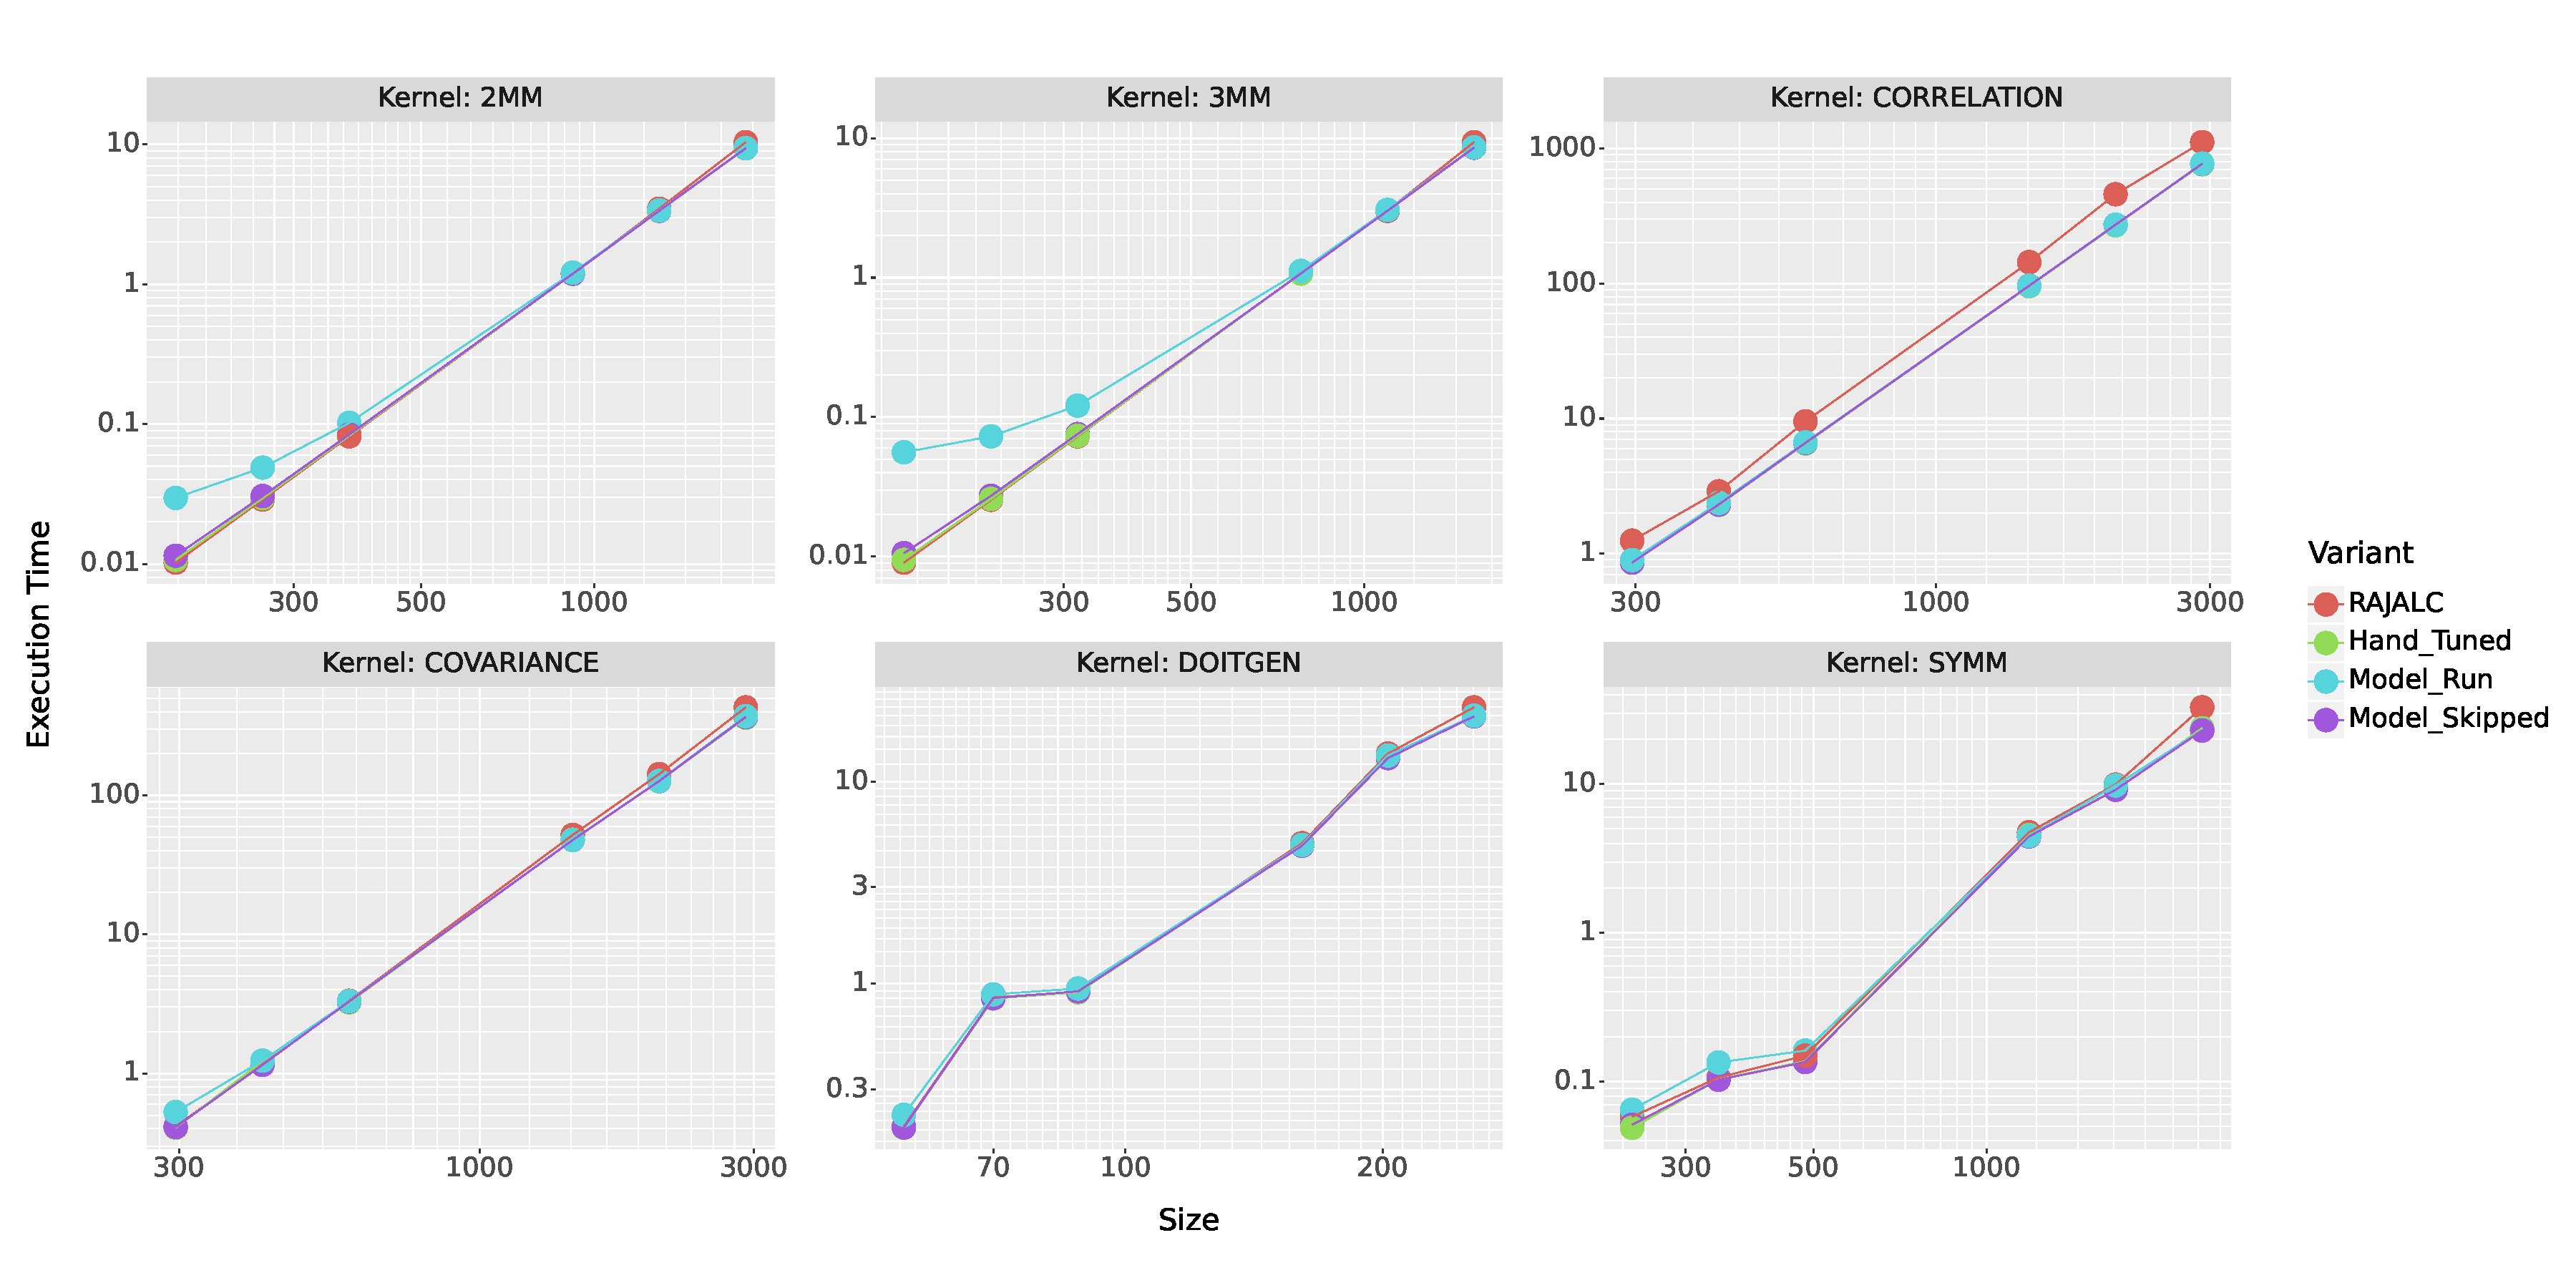
\includegraphics[width=\columnwidth]{lassen_speedups.pdf}
\caption{Execution times for evaluation on the Lassen system. Both axes are log-scale. Lower is better.}
\label{lassenSpeedups}
\end{figure}

Figure~\ref{quartzSpeedups} shows the execution times for the four variants on the Quartz system. 
For model accuracy, the only mismatches between the model-selected layout transformations and the hand-tuned heuristic selection were for the \textsc{3mm} variant.
For this benchmark, one of the target arrays, \verb.B., is only used in the first loop nest. 
Thus, the ``Hand Tuned'' variant converts to column-major before the first loop nest and back to row-major at the end of the entire loop chain.
The ILP model chooses to convert to column-major before the first loop nest, but immediately goes back to row-major instead of converting at the end of the loop chain.
Because the \verb.B. array is not used between the point the model chooses and the point the heuristic chooses, the difference does not affect the performance.

With regards to overhead, the ILP overhead (``Model Run'' vs ``Model Skipped'') was most significant for small problem sizes, especially for the \textsc{2mm}, \textsc{3mm}, \textsc{doitgen}, and \textsc{symm} kernels.
On average, for the smallest problem size, the modeling overhead was $387\%$ of the performance improvement achieved by the ``Hand Tuned'' variant.
This indicates that it is not possible to amortize the performance modeling cost for small problem sizes.
However, as the problem size increased, this overhead became less significant, as the solve time is constant no matter the problem size.
For the largest problem size, the modeling overhead was $23\%$ of the performance improvement of the ``Hand Tuned'' variant. 
The abstraction overhead (``Model Skipped'' vs ``Hand Tuned'') were negligible.
In some cases, especially for larger problem sizes, the ``Model Skipped'' variant slightly outperforms the ``Hand Tuned'' variant.
This is likely due to the highly templated nature of the code generated by the \FormatDecisions{} system allowing more aggressive compiler optimization.

Figure~\ref{lassenSpeedups} shows the results for the Lassen system.
The \textsc{3mm} benchmark produced the same mismatch between the heuristic choices and the model choices as on Quartz.
Otherwise, the model made the same choices as the heuristic-based approach.

Similar to the Quartz results, the ILP overhead was only significant for small problem sizes.
At the smallest size, the ILP overhead was $603\%$ of the performance improvement of the hand-tuned variant, meaning the ``Model Run'' variant took longer to execute that the baseline ``RAJALC'' variant.
The abstraction overhead was smaller, at $26\%$ of the performance improvement of the hand-tuned variant.
This means that it still saw performance improvement compared to the ``RAJALC'' variant, but less than the ``Hand Tuned'' variant.
For the largest problem size, the ILP overhead was much smaller, costing only $4.3\%$ of the hand-tuned performance improvement.
Like on Quartz, some benchmarks saw even greater performance improvements from using the \FormatDecisions{} abstraction without running the model.
On average, for the largest problem size, the ``Model Skipped'' variant saw $1.1\%$ improvement over the ``Hand Tuned'' variant.

\todo{move triangular iteration space piece here}
\section{Related Work}

The approach used in this chapter to provide library-level abstractions for layout transformations is most closely related to the inspector-executor pattern found in sparse computations~\cite{strout2018sparse}.
In codes with sparse data, the distribution of the nonzero data heavily influences the most performant schedule and data alyout, but is not known until runtime.
The inspector-executor pattern resolves this dilemma by breaking a computation into an inspector phase, which analyzes the structure of the data, and an executor phase, which uses the results to select from different possible implementations.
This approach has traditionally been used to aid in parallelizing sparse codes~\cite{ujaldon1996parallelization,fu1996run,venkat2016automating}.
However, it has also been used to select data transformations~\cite{venkat2015loop}.
\FormatDecisions' use of runtime performance modeling (inspecting) to determine the data layouts to use for the computation (executing) uses this pattern for a different class of computation.
It is also related to work on scheduling and data transformations, polyhedral compilation, and domain-specific languages.

\subsubsection{Schedule Transformations}
Early approaches to optimizing data locality use schedule transformations rather than data layout transformations. 
Work incorporated into the SUIF compiler uses interchange, reversal, skewing, and tiling~\cite{wolf1991data}, whereas Fortran source-to-source approaches also use loop fusion~\cite{mckinley1996improving}.
While schedule transformations avoid the overhead cost of layout conversion, their global nature can improve locality for one access while harming another.
Nevertheless, schedule transformations remain a popular approach to optimizing data locality and parallelism, 
especially through tiling techniques~\cite{bondhugula2008pluto,bertolacci2015parameterized,bondhugula2016diamond,bandishti2012tiling,unat2016tida}.

\subsubsection{Layout Transformation in HPF}
In the domain of data layout transformations, early work in High Performance Fortran (HPF) and D compilers~\cite{bixby1994automatic,kennedy1995automatic,kennedy1998automatic} provide foundations for a variety of later approaches.
Their framework follows a popular pattern: generate a space of possible choices, estimate the performance of different choices, and select an option using an ILP formulation. 
This chapter's ILP problem formulation is similar to theirs, although it does not use the data layout graph intermediate representation.
Furthermore, where their model for cost estimation focuses on communication costs in a distributed context, this approach models on-node performance costs of cache misses.

\subsubsection{Polyhedral Compilation}
The polyhedral model, traditionally used for schedule transformations, is commonly leveraged for data layout transformations as well.
With the rise of multicore chips, new strategies were needed to manage shared on-chip resources. 
Work by Lu et al.~\cite{lu2009data} and Zhang et al.~\cite{zhang2011optimizing} develop layout optimization schemes based on the polyhedral model and use a combination of strip-mining, permutation, and padding transformations.

\subsubsection{Heterogenous Computing}
Data layout transformation frameworks are also popular for heterogeneous programming systems, especially for stencil codes.
Sung, Stratton, and Hwu~\cite{sung2010data} use data layout transformations to relieve pressure on memory controllers in structured grid applications by spreading data out across the address space based on the indexing behavior of the application.
Henretty et al.~\cite{henretty2011data} develop a layout transformation and accompanying static analysis to address stream alignment conflicts for SIMD architectures.
Jaeger and Barthou~\cite{jaeger2012automatic} present a strategy for generating stencil codes with optimal data layouts using a multi-padding layout transformation.
Recognizing the need for specialized support for ever-changing chip structure, Majeti et al.~\cite{majeti2013compiler} develop a programmer (or autotuner) guided data transformation system.
Built into the Habenero-C compiler, the meta-data provided by the user guides the generation of architecture-specific SOA, AOS, and SOAOS data layouts.
Another approach by Kofler, Cosenza, and Fahringer~\cite{kofler2015automatic} convert AOS implementations to other data layouts for GPU applications automatically.  
With the exception of Majeti et al., these approaches do not provide an interface to the developer, and without exception are compiler-based approaches.
This approach presents an interface to the developer in the form of a library API, allowing user control and low-cost integration into existing workloads.

\subsubsection{Pragmas}
Although still in the realm of the compiler-based techniques, pragmas have been suggested as a solution to the problem of providing control over the transformations to the user.
Proposals to add such pragmas have been submitted to OpenMP~\cite{kruse2019design} and Clang~\cite{kruse2018user}.
Other work has implemented transformation pragmas into a source-to-source compiler~\cite{xu2014semi}. 

\subsubsection{Domain-Specific Languages}
Domain-specific language approaches are another avenue for presenting users with control of the data layout transformations to apply. 
Kronawitter et al.~\cite{kronawitter2018automatic} incorporate data layout specifications into the ExaSlang DSL.
Using a polyhedral framework, the Tiramisu DSL~\cite{baghdadi2019tiramisu} also enables data layout transformation specifications.
In constrast to these specialized approaches, the approach here seeks to support a wider class of computations without needing the additional machinery required to use DSLs. 


\section{Conclusion}

Effective use of the memory hierarchy is critical to application performance.
One way of doing this is by changing how data is stored within memory.
Yet, in performance portability libraries like RAJA and Kokkos, where one codebase is used for machines with different architectures, there are not yet tools for transforming the layout of data between parts of a computation. 
Thus, if a developer wants to introduce these optimizations, they are left in a time-consuming, error-prone situation --- further exacerbated by the potential for data layout transformations to not be worth the overhead.

\FormatDecisions remedies this situation by combining a declarative format specification interface with an automated decision model.
Integrated directly into the performance portability library RAJA, but possible in any library with computation objects and a data View-like abstraction, \FormatDecisions{} provides a flexible interface for quick exploration of data layout changes. 
Additionally, \FormatDecisions{} uses an ILP formulation to optionally identify other profitable transformations, \enquote{filling in} the user specification.

When evaluated against hand-implemented layout transformations on six benchmark kernels, \FormatDecisions{} provides comparable performance improvements for sufficiently large problem sizes with a fraction of the code changes.
Furthermore, subsequent modifications to the layout transformations, for example as part of porting a codebase to a new machine, are reduced to single-line changes. 
This improves maintainability and reduces the potential for introducing bugs.
Combined with the support for schedule transformations introduced in Chapter 2, performance portability library users can maintainably optimize a wide range of computations. 
The next chapter explores widening this range of supported computations even further.
